\chapter{Introduzione alla Dependability e agli Standard relativi al settore ferroviario}

I sistemi informatici complessi, ovvero tutti quei sistemi composti da sottosistemi indipendenti in grado di interagire fra loro, vengono adoperati sempre pi� frequentemente per svolgere compiti
altamente critici, che compromettono la sicurezza e l'incolumit� delle persone.
Si pensi per esempio ai sistemi di controllo di aerei, delle centrali nucleari o ai sistemi ferroviari.
� di fondamentale importanza che tali sistemi adottino delle tecniche in grado di mantenere sempre corrette le funzioni per le quali sono destinati.\\
La \textbf{dependability} � una caratteristica dei sistemi e consiste nella loro capacit� di mostrarsi "affidabili" nei confronti degli utilizzatori, tale caratteristica porta gli utilizzatori a potersi "fidare" del sistema stesso e a poterlo quindi utilizzare senza particolari preoccupazioni.\cite{sei}
La dependability � un concetto che comprende all'interno del suo significato i seguenti attributi:
\begin{itemize}

\item Disponibilit� (\textit{Availability}): � la prontezza del sistema nell'erogare un servizio corretto; misura la fornitura di servizio corretto, rispetto all'alternanza tra servizio corretto e non corretto.
\item Affidabilit� (\textit{Reliability}): � la capacit� del sistema di erogare un servizio corretto in modo continuo, misura la fornitura continua di un servizio corretto.
\item Confidenzialit� (Confidentiality): � l'assenza di diffusione non autorizzata di informazioni; misura l'assenza di esposizione non autorizzata di informazione.

\item Manutenibilit� (\textit{Mantainability}): la capacit� del sistema di subire modifiche e riparazioni; misura il tempo necessario per ristabilire un servizio corretto.
\item Sicurezza (\textit{Safety}): � l'assenza di conseguenze catastrofiche sull'utente e sull'ambiente circostante.
\item Sicurezza (\textit{Security}): � vista come la contemporanea esistenza di availability, confidentiality e integrity. \cite{sei}
\end{itemize}
Ciascuno di questi attributi pu� essere pi� o meno importante in base all'applicazione: la disponibilit� del servizio � sempre richiesta, anche se pu� variare sia l'importanza relativa che il livello quantitativo richiesto; la affidabilit�, la sicurezza, la confidenzialit� e gli altri attributi possono essere richiesti o meno.\\
Il grado con cui un sistema possiede questi attributi deve essere interpretato in senso probabilistico e non in senso assoluto, deterministico; a causa dell'inevitabile occorrenza dei guasti i sistemi non sono mai totalmente disponibili, affidabili, safe o secure. Per questo gli attributi di dependability possono essere definiti in senso probabilistico cos� da poterli trattare in modo quantitativo. \cite{sei}
Lo sviluppo di sistemi dependable richiede l'utilizzo combinato di quattro tipologie di tecniche:
\begin{itemize}
	\item \textbf{Prevenzione dei guasti}: per prevenire l'occorrenza o introduzione di guasti nel sistema;
	\item \textbf{Tolleranza ai guasti}: per erogare un servizio corretto anche in presenza di guasti;
	\item \textbf{Rimozione dei guasti}: per ridurre il numero o la gravit� dei guasti;
	\item \textbf{Previsione dei guasti}: per stimare il numero di guasti presenti nel sistema, la loro incidenza futura o le loro probabili conseguenze.\cite{due}
\end{itemize}
I sistemi informatici forniscono servizi sempre pi� sofisticati e per questo richiedono standard qualitativi sempre pi� elevati.\\ Nel \textbf{settore ferroviario} le principali normative che sono state varate in ambito europeo sono le seguenti: 
\begin{itemize}
	\item EN 50126: stabilisce delle linee guida per la realizzazione dell'attivit� RAMS (Reliability-Availability-Mantainability-Safety) lungo tutto il ciclo di vita di un prodotto ferroviaro. Questa normativa � da ritenersi applicabile ad agni tipo di prodotto destinato ad operare nel settore ferroviario, si tratti di un impianto fisso, di un treno oppure anche solo di un impianto che lo compone. Dato il suo carattere generale, la normativa non d� elementi specifici n� tantomeno esprime requisiti quantitativi. \cite{tredici}
	\item EN 50128: relativa allo sviluppo di software per applicazioni di sicurezza. \cite{undici}
	\item EN 50129: inerente allo sviluppo di apparecchiature elettriche/elettroniche di sicurezza per il segnalamento ferroviario.
	\item EN 50121: riguarda le relazioni tra i sistemi ferroviari ed il mondo esterno, con particolare riguardo alla compatibilit� elettromagnetica. 
	\item EN 50155: inerente le condizioni del materiale elettico utilizzato nelle fasi di sviluppo, costruzione e testing. 
	\item EN 50159: affronta invece la sicurezza delle comunicazioni in ambito ferroviario \cite{dodici}. 
\end{itemize}
\begin{figure}
	\centering
	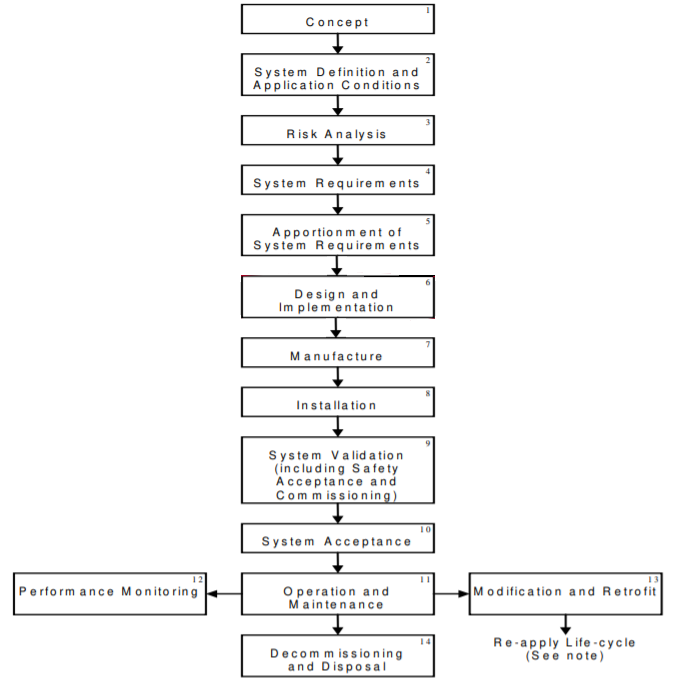
\includegraphics[scale=0.8]{img/diagstandard}
	\caption{Diagramma EN 50 126 \cite{tredici}}
\end{figure}
Nel diagramma sono riportate le fasi del ciclo di vita relative alla normativa EN50126. 
 Le prime fasi hanno come obiettivo quello di definire le funzioni del sistema, l'interazione con l'ambiente esterno e le interfacce. Inoltre devono essere pianificate le attivit� di safety e di verifica e validazione. Le normative EN50128 e EN50129 vengono utilizzate in particolare nella fase 6 (Design and implementation): in questa fase viene definita l'architettura dei sottosistemi e inoltre viene affrontato lo sviluppo hardware e software.\cite{undici}\\
 Lo standard EN50126 descrive gli elementi chiave che devono essere definiti per gestire la safety di un sistema:
 \begin{itemize}
 	\item politica generale sulla safety;
 	\item piano di safety;
 	\item registro degli azzardi;
 	\item controlli interni al sistema;
 	\item sistema per riportare i fallimenti;
 	\item sistema per la gestione delle azioni correttive;
 	\item processo di valutazione dei rischi per individuare gli azzardi.
 \end{itemize}
Tale normativa, come tante altre in diversi ambiti, richiede che prima che il sistema inizi a operare, tutti i rischi siano stati misurati e valutati e che siano considerati tollerabili.\cite{tredici}\\ 
Il rischio � quindi l'unit� di misura del sistema di gestione della safety. Misurare un rischio non � semplice, non esiste infatti uno strumento diretto per effettuare tale operazione. E' possibile per� utilizzare due approcci indiretti:
\begin{itemize}
	\item la statistica, per misurare i rischi del passato;
	\item l'hazard analysis, per predirre i rischi del futuro.
\end{itemize}
Ovviamente la nostra attenzione si concentra sull'analisi dei rischi, con lo scopo di evidenziare le problematiche a cui un certo sistema pu� andare incontro. 
\newline
\section{SIL - Safety Integrity Level}
 

Un'altra normativa che � opportuno riportare � la IEC 61508 (Sicurezza funzionale di sistemi Elettrici/Elettronici/Elettronici Programmabili), applicabile ai pi� svariati settori industriali, dal settore dell'industria di processo (ad esempio chimico e petrolchimico), ai macchinari, al settore dei trasporti. La norma IEC 61508 definisce quattro livelli di Safety Integrity Level (da SIL1 a
SIL4), ciascuno dei quali definisce una misura quantitativa della necessaria
riduzione del rischio e quindi il grado di affidabilit� che il sistema di sicurezza
deve raggiungere per poter garantire tale riduzione.\\
Nella norma sono definiti i metodi per la determinazione del PFD (Probability of Failure on Demand) o PFH (Probability of Failure per Hour) e del RRF (Risk Reduction Factor), utilizzati durante la classificazione SIL. \cite{quindici}
\begin{figure}[ht]
	\centering
	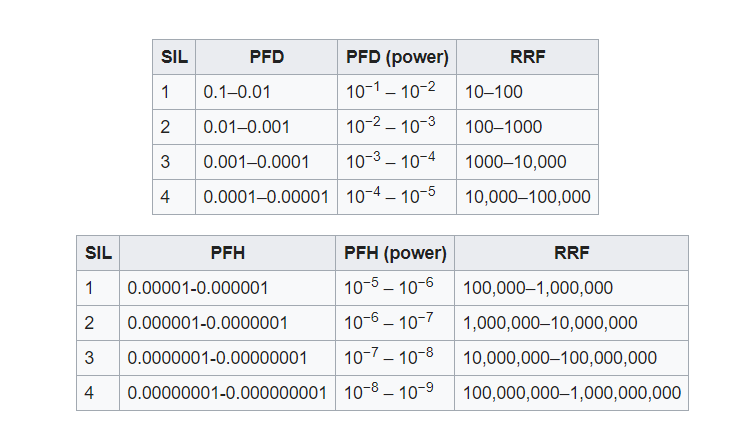
\includegraphics[scale=0.7]{img/sil}
	\caption{Classificazione SIL \cite{quindici}}
\end{figure}
